\documentclass[11pt, oneside]{article}   	% use "amsart" instead of "article" for AMSLaTeX format

\usepackage{geometry}
 \geometry{
 a4paper,
 total={170mm,257mm},
 left=20mm,
 top=30mm,
 bottom=25mm, 
 }
 
%\usepackage{geometry}                		% See geometry.pdf to learn the layout options. There are lots.
%\geometry{letterpaper}                   		% ... or a4paper or a5paper or ... 
%\geometry{landscape}                		% Activate for rotated page geometry
%\usepackage[parfill]{parskip}    		% Activate to begin paragraphs with an empty line rather than an indent
\usepackage{graphicx}				% Use pdf, png, jpg, or eps§ with pdflatex; use eps in DVI mode
								% TeX will automatically convert eps --> pdf in pdflatex		

\usepackage{amssymb}
\usepackage{amsmath}
\usepackage{amsthm}
\usepackage{fancyhdr}
\usepackage[utf8]{inputenc}
\usepackage[english]{babel}
\usepackage{enumerate}
\usepackage{arcs}
\usepackage{array}
\usepackage{tabularx} 
\usepackage{tikz}
%SetFonts

%SetFonts

\usepackage[inline]{asymptote}


\pagestyle{fancy}
\fancyhf{}
\lhead{Name: \textbf{William Zhong}, Username: \textbf{wzsuperb}, ID: \textbf{40819}}
\rhead{USAMTS, year 33, round 3}
\rfoot{December, 2021}


%\title{In-class Quiz}
%\author{Teacher David}
%\date{}							% Activate to display a given date or no date

\begin{document}
%\maketitle

\section{Problem 1/3/33}
\vspace{20pt}

\begin{center}
\begin{asy}
size(5cm);
for (int i=0; i<7; ++i) {
  dot((i,0));
}

for (int i=1; i<6; ++i) {
  dot((i,-1));
}

for (int i=0; i<7; ++i) {
  dot((i,-2));
}

for (int i=0; i<6; ++i) {
  dot((i,-3));
}

for (int i=0; i<7; ++i) {
  dot((i,-4));dot((i,-5));
}

dot((0,-6)); dot((1,-6));
dot((3,-6)); dot((4,-6));dot((5,-6));

draw((0,0)--(3,0));
draw((4,0)--(6,0));

draw((1,0)--(1,-1));
draw((2,0)--(2,-3));
draw((5,0)--(5,-5));
draw((2,-1)--(3,-1));
draw((5,-1)--(4,-1));
draw((2,-2)--(3,-2));
draw((5,-2)--(6,-2));
draw((0,-2)--(0,-6));
draw((1,-2)--(1,-3));
draw((4,-2)--(4,-3));
draw((0,-3)--(5,-3));
draw((3,-3)--(3,-5));
draw((0,-4)--(1,-4));
draw((2,-4)--(3,-4));
draw((5,-4)--(6,-4));
draw((4,-4)--(4,-6));
draw((0,-5)--(2,-5));
draw((4,-5)--(6,-5));
draw((1,-5)--(1,-6));
draw((3,-6)--(5,-6));
\end{asy}
\end{center}

\newpage
\section{Problem 2/3/33}

\begin{center}
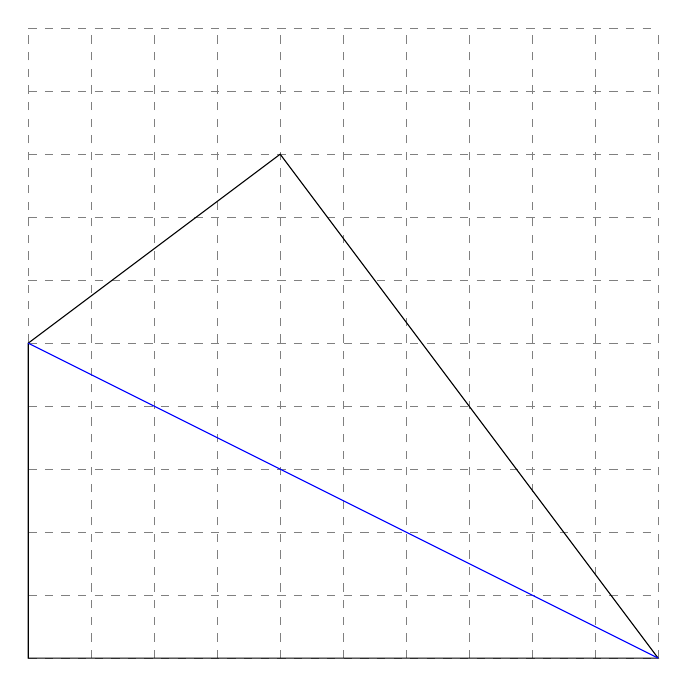
\begin{tikzpicture}[scale=.8]
\draw[dashed, gray] (0,0) grid (10,10);
\draw (0,0) -- (0,5) -- (4,8) -- (10,0)--cycle;
\draw [blue] (0,5) -- (10,0);
\end{tikzpicture}
\end{center}

\newpage
\section{Problem 3/3/33}
Given a grid of size $n\times n$, the number of double staircases is $4^{n-1}$.\\

\begin{proof}

Some simple observations: if $n=1$, there is $1$ double staircase; if $n=2$, there are $4$ double staircases. 


Given an $n\times n$ grid, suppose $T=\{T_1, T_2, \cdots, T_k\}$, for any $T_i \in T$, we can transform it into a double staircase for grid of size $(n-1)\times (n-1)$ by removing the longest column from $T_i$. Vertically, the transformation only removes one rectangle of dimensions $n\times 1$ from $T_i$. Horizontally, every rectangle of size $1\times j$ $(2\le j \le n)$ will be reduced to a rectangle of size $1\times (j-1)$, and the original rectangle of size $1\times 1$ is removed. 

Conversely, we can transform $T_i$ to form a double staircase for a grid of size $(n+1)\times (n+1)$. The transformation is done by adding a column of size $(n+1)\times 1$ to $T_i$, given that horizontally the new column must be added adjacent to the longest column, and  vertically the new column should match the top or the bottom of the grid. Vertically, this transformation adds a rectangle of size $(n+1)\times 1$ to $T_i$. Horizontally, every rectangle of size $1\times j (1\le j \le n)$ will be increased to a rectangle of size $1\times (j+1)$. Since the new column is of size $n+1$, it is one block longer than the original longest column of $T_i$ , adding it to $T_i$ will create a rectangle of size $1\times1$ under horizontal partition.

Suppose the longest column of $T_i$ is $C$. There are 4 ways of transforming $T_i$ into a double staircase for a grid of size $(n+1)\times (n+1)$: 
\begin{enumerate}
\item Placing the new column adjacent to the east of $C$ and match the bottom of $C$; 
\item Placing the new column adjacent to the east of $C$ and match the top of $C$; 
\item Placing the new column adjacent to the west of $C$ and match the bottom of $C$; 
\item Placing the new column adjacent to the west of $C$ and match the top of $C$.
\end{enumerate}

All double staircases for grid of size $(n+1)\times (n+1)$ can be transformed from $T_i $ $(T_i\in T)$. Given any $T_j \ne T_i$, the staircases transformed from $T_j$ should be different from those transformed from $T_i$. 

Assume there are $f(x)$ double staircases for a grid of size $x\times x$, we have $f(1)= 1$. Every double staircase can be transformed into 4 different staircases for a grid of size $(x+1)\times (x+1)$, then $f(x+1) = 4f(x)$. 

Therefore, 
\[f(n)= 4f(n-1) = 4^{n-1} f(1)=4^{n-1}.\]

\end{proof}






\end{document}  